\chapter{Planificación y coste}
Este capítulo trata sobre la planificación llevada a cabo y el coste total de la implementación. Con respecto a la planificación se explica tanto la planificación llevada con los tutores responsables de dicho proyecto como la planificación personal a la hora de desarrollar el proyecto.

\section{Planificación}
La planificación de este proyecto comenzó con una reunión a finales de noviembre de 2019, para tratar el problema a resolver. La reunión fue llevada a cabo por Miguel Damas Hermoso, Oresti Baños Legrán, ambos tutores de este proyecto e Ignacio Díaz Reyes, CEO de mDurance, empresa encargada de aportar todas las herramientas necesarias para la toma de datos, así como, los datos en cuestión para la realización de este proyecto.
En esta reunión se debatió sobre la temática del proyecto y sobre lo que se intentaba aportar con dicha solución. También se comentó el "dataset" que iba a ser utilizado para el estudio, el cuál se iba a encargar de tomar un centro de Barcelona que trabajaba junto a mDurance.

Para finalizar se me realizó una prueba con la herramienta que iba a ser utilizada para medir las señales de electromiografía para ver como funcionaba y aumentar mi conocimiento sobre el tema.

A continuación se explica el restante de las reuniones llevadas a cabo y la planificación personal a la hora de desarrollar el proyecto.

\subsection{Sesiones formativas y reuniones}

Con respecto a la adquisición de conocimientos sobre electromiografía, toma de datos, filtración y amplificación de las señales tomadas, recibí dos sesiones formativas en el centro de mDurance de aproximadamente dos horas. En estas reuniones Ignacio Díaz Reyes realizó una introducción hacia la electromiografía y de sus aplicaciones en el mundo actual. A parte de esto, también nos habló sobre las diferentes características de las señales, sobre todo de las más conocidas y utilizadas en la actualidad.
Esto fue complementado mostrando análisis realizados sobre pacientes para ver como se puede diagnosticar ciertos déficits en la musculatura solo con extraer características de las señales EMG. Por último comentar que me facilitó documentación sobre la EMG y sobre sus características, tanto en el dominio del tiempo como en el dominio de la frecuencia.

Después de estas dos sesiones, que se realizaron el 21 de enero y el 11 de febrero de 2020, ya estaba preparado para empezar el proyecto en la fase de extracción de características de la señal EMG.

La próxima reunión que realizamos fue por medio de GoogleMet, ya que había un problema con los datos que supuestamente iban a ser utilizados para el proyecto. Debido al COVID-19 y a la declaración del estado de alarma, dichos datos no pudieron ser tomados, por lo que nos encontrábamos a mitad de marzo y sin datos para poder realizar el proyecto. Esta reunión fue clave para poder realizar el proyecto. En ella, ambos tutores, junto con Ignacio y Carlos, el fisioterapeuta de mDurance, hicimos una puesta en común de ideas para poder obtener otro "dataset" que supliera al original. Se acordó realizar una búsqueda sobre posibles ideas y zanjar el problema en una próxima reunión.

En la siguiente reunión, unos tres días posterior a la anterior, Ignacio aportó una solución, ya que había hablado con un colaborador que se iba a encargar de tomar un nuevo "dataset". Esta nueva orientación era muy parecida a la original, solo que añadía una nueva idea, la fatiga. Con esto además de hallar que pacientes sufrían de rodilla lesionada, también podía ser utilizado para detectar la fatiga muscular. Este "dataset" trataba sobre un ejercicio multiarticular, la sentadilla. Se acordó que dispondría de los datos en la mayor brevedad posible. Finalmente tuve acceso a parte de los datos el 24 de mayo y el 20 de junio a la totalidad de ellos. Por lo que esto implicó la imposibilidad de poder presentar el proyecto en la primera convocatoria.

Una vez que ya disponía de los datos, a partir del 13 de julio, tuve reuniones consecutivas con ambos tutores, para ir mostrándoles como iba el desarrollo del proyecto e ir acordando el formato de la memoria y todo lo que debía de añadir.

El 27 de julio tuvimos una ultima reunión donde les mostré un prototipo bastante avanzado del desarrollo, el cual, vieron bastante bien, y se acordó que ya solo tenía que desarrollar el proyecto final y complejo, así como el desarrollo de la memoria. 

Para la memoria se acordó enviar un prototipo para mediados de agosto, y la memoria final para el 3 de septiembre, para así tener siempre un margen de error y poder corregir posibles errores antes de la entrega final de los proyectos.

Con respecto a mi propio trabajo, se comenta en la siguiente sección. 

\subsection{Implementación y memoria}

Una vez realizadas las dos sesiones formativas de EMG comentadas anteriormente, ya podía empezar a indagar en el tema de la electromiografía y su análisis de datos. Durante los meses de enero, febrero y marzo, debido a la incertidumbre de los datos explicada, tuve acceso a unas señales EMG de prueba facilitadas por mDurance para poder hacer el desarrollo de la extracción de las características. Durante estos meses fui obteniendo más conocimientos sobre las señales de EMG, sus características y utilidad, así como, sobre la clasificación binaria de dichas señales. Además con los datos de prueba, pude realizar la implementación de los algoritmos de extracción de características que yo consideré más relevantes para la realización de este proyecto.

A partir del 24 de mayo, cuando recibí la primera parte del dataset final, debido a que la fase de extracción de características ya la tenía realizada, me dediqué a indagar sobre el tema de clasificación de señales usando librerías de Python, y a investigar que algoritmo de selección de características era el más indicado para obtener un mejor rendimiento en este proyecto.

Durante las reuniones de julio, mis tutores fueron orientándome sobre el trabajo que iba realizando, y así el 27 de julio pude tener un prototipo, al que sólo sería necesario añadirle más complementos para que fuese el resultado final. Con todo esto para el 3 de agosto, ya tuve una versión final del proyecto y empecé el desarrollo de la memoria del proyecto.


\begin{figure}[ht]
\centering
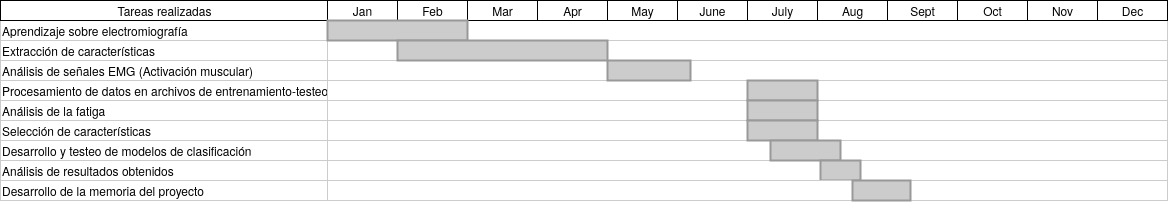
\includegraphics[width=1.0\textwidth,height=4cm]{imagenes/tareas realizadas.png}
\caption{ Diagrama de Gantt sobre el trabajo personal }
\label{fig:gantt}
\end{figure}



\section{Coste}
Una vez realizado el estudio sobre la clasificación y viendo cual sería el mejor clasificador que resolviese el problema, el siguiente paso sería llevarlo al mercado. Habría que realizar una aplicación móvil, conectada a dicho sensor para que mientras se tome los datos, un programa paralelo los analice y nos de los resultados de la fatiga en el tiempo de ejecución, intentando una eficiencia máxima y el mínimo tiempo de procesamiento de datos. Para realizar dicho trabajo los costes se podrían dividir entre el coste de la tecnología utilizada para la obtención de los datos y el coste de los recursos humanos encargados de desarrollar el software.

\subsection{Tecnología utilizada}
Con respecto al precio de la tecnología utilizada, para la medición de los datos se ha utilizado el sensor de mDurance. Se han evaluado ambas rodillas a la hora de realizar una sentadilla por lo que se ha hecho uso del mDurance Premium de 4 canales (Ver Imagen \ref{fig:mDurance}), que además también incluye un sensor para medir el rango de movimiento de cada repetición. Esta herramienta tiene un coste actual de 5.445 \euro \thinspace\thinspace(Enlace a tienda \cite{informacionPreciomdurance}).

\begin{figure}[ht]
\centering
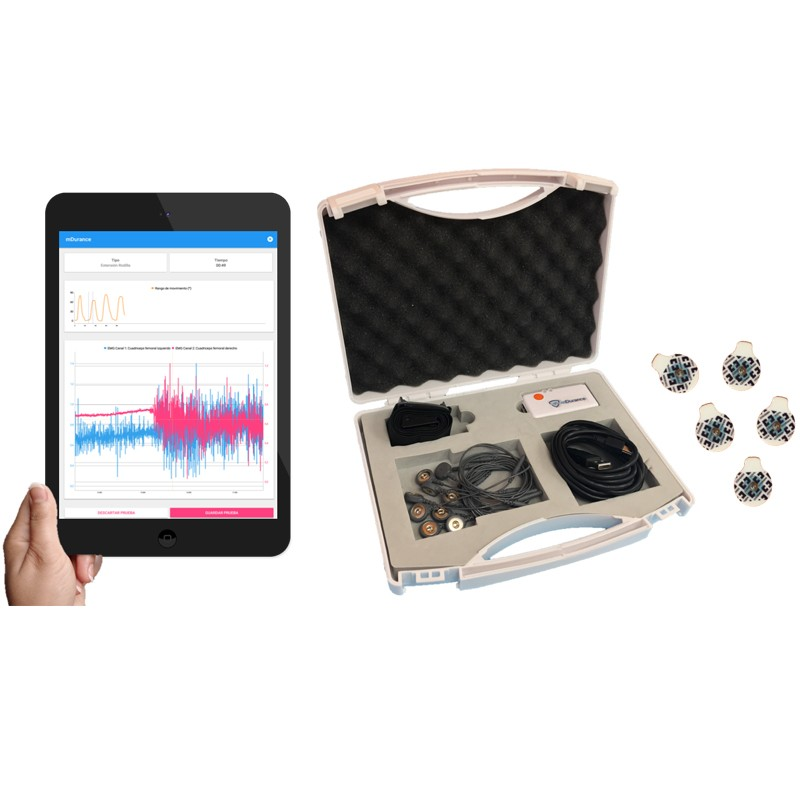
\includegraphics[scale=0.3]{imagenes/electromiografo-de-superficie-de-dos-canales-mdurance-pro.jpg}
\caption{ Electromiógrafo mDurance \cite{electrodosMdurance}}
\label{fig:mDurance}
\end{figure}

\subsection{Recursos humanos}
Para el desarrollo software de la aplicación un ingeniero informático especializado en el desarrollo y la implementación de software cobra unos 2000 \euro/mes  \cite{salarioinformatico}. Estimo que el desarrollo de dicha aplicación se podría llevar a cabo en 2 meses de trabajo, teniendo en cuenta un testeo de funcionamiento para que no requiera un gran mantenimiento al tener la mayoría de errores depurados.

A este precio habría que añadirle lo que cobra un fisioterapeuta/entrenador que será el encargado de tomar los datos a sus clientes. El sueldo medio en España de un fisioterapeuta es de 1217 \euro/mes \cite{salariofisio}.

El precio total de los recursos humanos seria de unos 5217 \euro, debido a dos meses de trabajo del ingeniero informático y a un mes de trabajo del fisioterapeuta encargado de la toma de datos para haber podido realizar el estudio sobre que clasificador es el que obtiene mejores prestaciones.

\subsection{Precio del servicio final}

Todo esto haría un presupuesto final de unos 10662 \euro, un precio bastante elevado, pero si lo analizamos muy rentable, ya que se trata de una herramienta pionera en el sector, que si se desarrolla de la forma adecuada de seguro que sería utilizada por una gran cantidad de atletas y dejaría grandes beneficios.

Este software podría ser implementado dentro de la herramienta base de mDurance, aportando así una funcionalidad extra.


\begin{figure}[ht]
\centering
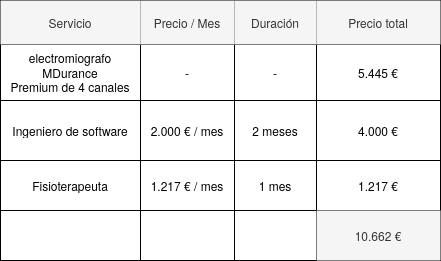
\includegraphics[scale=0.6]{imagenes/precio total.png}
\caption{ Desglose de los precios del proyecto}
\label{fig:precios}
\end{figure}






